% Options for packages loaded elsewhere
\PassOptionsToPackage{unicode}{hyperref}
\PassOptionsToPackage{hyphens}{url}
%
\documentclass[
]{article}
\usepackage{amsmath,amssymb}
\usepackage{lmodern}
\usepackage{iftex}
\ifPDFTeX
  \usepackage[T1]{fontenc}
  \usepackage[utf8]{inputenc}
  \usepackage{textcomp} % provide euro and other symbols
\else % if luatex or xetex
  \usepackage{unicode-math}
  \defaultfontfeatures{Scale=MatchLowercase}
  \defaultfontfeatures[\rmfamily]{Ligatures=TeX,Scale=1}
\fi
% Use upquote if available, for straight quotes in verbatim environments
\IfFileExists{upquote.sty}{\usepackage{upquote}}{}
\IfFileExists{microtype.sty}{% use microtype if available
  \usepackage[]{microtype}
  \UseMicrotypeSet[protrusion]{basicmath} % disable protrusion for tt fonts
}{}
\makeatletter
\@ifundefined{KOMAClassName}{% if non-KOMA class
  \IfFileExists{parskip.sty}{%
    \usepackage{parskip}
  }{% else
    \setlength{\parindent}{0pt}
    \setlength{\parskip}{6pt plus 2pt minus 1pt}}
}{% if KOMA class
  \KOMAoptions{parskip=half}}
\makeatother
\usepackage{xcolor}
\usepackage[margin=1in]{geometry}
\usepackage{color}
\usepackage{fancyvrb}
\newcommand{\VerbBar}{|}
\newcommand{\VERB}{\Verb[commandchars=\\\{\}]}
\DefineVerbatimEnvironment{Highlighting}{Verbatim}{commandchars=\\\{\}}
% Add ',fontsize=\small' for more characters per line
\usepackage{framed}
\definecolor{shadecolor}{RGB}{248,248,248}
\newenvironment{Shaded}{\begin{snugshade}}{\end{snugshade}}
\newcommand{\AlertTok}[1]{\textcolor[rgb]{0.94,0.16,0.16}{#1}}
\newcommand{\AnnotationTok}[1]{\textcolor[rgb]{0.56,0.35,0.01}{\textbf{\textit{#1}}}}
\newcommand{\AttributeTok}[1]{\textcolor[rgb]{0.77,0.63,0.00}{#1}}
\newcommand{\BaseNTok}[1]{\textcolor[rgb]{0.00,0.00,0.81}{#1}}
\newcommand{\BuiltInTok}[1]{#1}
\newcommand{\CharTok}[1]{\textcolor[rgb]{0.31,0.60,0.02}{#1}}
\newcommand{\CommentTok}[1]{\textcolor[rgb]{0.56,0.35,0.01}{\textit{#1}}}
\newcommand{\CommentVarTok}[1]{\textcolor[rgb]{0.56,0.35,0.01}{\textbf{\textit{#1}}}}
\newcommand{\ConstantTok}[1]{\textcolor[rgb]{0.00,0.00,0.00}{#1}}
\newcommand{\ControlFlowTok}[1]{\textcolor[rgb]{0.13,0.29,0.53}{\textbf{#1}}}
\newcommand{\DataTypeTok}[1]{\textcolor[rgb]{0.13,0.29,0.53}{#1}}
\newcommand{\DecValTok}[1]{\textcolor[rgb]{0.00,0.00,0.81}{#1}}
\newcommand{\DocumentationTok}[1]{\textcolor[rgb]{0.56,0.35,0.01}{\textbf{\textit{#1}}}}
\newcommand{\ErrorTok}[1]{\textcolor[rgb]{0.64,0.00,0.00}{\textbf{#1}}}
\newcommand{\ExtensionTok}[1]{#1}
\newcommand{\FloatTok}[1]{\textcolor[rgb]{0.00,0.00,0.81}{#1}}
\newcommand{\FunctionTok}[1]{\textcolor[rgb]{0.00,0.00,0.00}{#1}}
\newcommand{\ImportTok}[1]{#1}
\newcommand{\InformationTok}[1]{\textcolor[rgb]{0.56,0.35,0.01}{\textbf{\textit{#1}}}}
\newcommand{\KeywordTok}[1]{\textcolor[rgb]{0.13,0.29,0.53}{\textbf{#1}}}
\newcommand{\NormalTok}[1]{#1}
\newcommand{\OperatorTok}[1]{\textcolor[rgb]{0.81,0.36,0.00}{\textbf{#1}}}
\newcommand{\OtherTok}[1]{\textcolor[rgb]{0.56,0.35,0.01}{#1}}
\newcommand{\PreprocessorTok}[1]{\textcolor[rgb]{0.56,0.35,0.01}{\textit{#1}}}
\newcommand{\RegionMarkerTok}[1]{#1}
\newcommand{\SpecialCharTok}[1]{\textcolor[rgb]{0.00,0.00,0.00}{#1}}
\newcommand{\SpecialStringTok}[1]{\textcolor[rgb]{0.31,0.60,0.02}{#1}}
\newcommand{\StringTok}[1]{\textcolor[rgb]{0.31,0.60,0.02}{#1}}
\newcommand{\VariableTok}[1]{\textcolor[rgb]{0.00,0.00,0.00}{#1}}
\newcommand{\VerbatimStringTok}[1]{\textcolor[rgb]{0.31,0.60,0.02}{#1}}
\newcommand{\WarningTok}[1]{\textcolor[rgb]{0.56,0.35,0.01}{\textbf{\textit{#1}}}}
\usepackage{graphicx}
\makeatletter
\def\maxwidth{\ifdim\Gin@nat@width>\linewidth\linewidth\else\Gin@nat@width\fi}
\def\maxheight{\ifdim\Gin@nat@height>\textheight\textheight\else\Gin@nat@height\fi}
\makeatother
% Scale images if necessary, so that they will not overflow the page
% margins by default, and it is still possible to overwrite the defaults
% using explicit options in \includegraphics[width, height, ...]{}
\setkeys{Gin}{width=\maxwidth,height=\maxheight,keepaspectratio}
% Set default figure placement to htbp
\makeatletter
\def\fps@figure{htbp}
\makeatother
\setlength{\emergencystretch}{3em} % prevent overfull lines
\providecommand{\tightlist}{%
  \setlength{\itemsep}{0pt}\setlength{\parskip}{0pt}}
\setcounter{secnumdepth}{-\maxdimen} % remove section numbering
\usepackage{float}
\usepackage{pgf}
\usepackage{forest}
\usepackage{caption}
\usepackage{pict2e}
\usepackage{lipsum}
\usepackage{amsthm}
\usepackage{tikz}
\ifLuaTeX
  \usepackage{selnolig}  % disable illegal ligatures
\fi
\IfFileExists{bookmark.sty}{\usepackage{bookmark}}{\usepackage{hyperref}}
\IfFileExists{xurl.sty}{\usepackage{xurl}}{} % add URL line breaks if available
\urlstyle{same} % disable monospaced font for URLs
\hypersetup{
  pdftitle={texessai},
  pdfauthor={st.},
  hidelinks,
  pdfcreator={LaTeX via pandoc}}

\title{texessai}
\author{st.}
\date{2023-01-04}

\begin{document}
\maketitle

this script works, packages included in yaml header\\
TODO not working: figure captions, inclusion of external .tex
configuration, html output - MIND: restore githistory commented ``wks.''
for working output configurations

\begin{Shaded}
\begin{Highlighting}[]
\NormalTok{knitr}\SpecialCharTok{::}\NormalTok{opts\_chunk}\SpecialCharTok{$}\FunctionTok{set}\NormalTok{(}\AttributeTok{echo =} \ConstantTok{TRUE}\NormalTok{)}
\FunctionTok{options}\NormalTok{(}\AttributeTok{tinytex.verbose =} \ConstantTok{TRUE}\NormalTok{,}\AttributeTok{engine=}\StringTok{"lualatex"}\NormalTok{)}

\FunctionTok{library}\NormalTok{(tinytex)}
\end{Highlighting}
\end{Shaded}

\begin{verbatim}
## Warning: package 'tinytex' was built under R version 4.1.2
\end{verbatim}

\begin{Shaded}
\begin{Highlighting}[]
\CommentTok{\#library(knitr)}
\FunctionTok{library}\NormalTok{(tikzDevice)}
\FunctionTok{check\_installed}\NormalTok{(}\StringTok{"forest"}\NormalTok{)}
\end{Highlighting}
\end{Shaded}

\begin{verbatim}
## [1] TRUE
\end{verbatim}

\begin{Shaded}
\begin{Highlighting}[]
\FunctionTok{check\_installed}\NormalTok{(}\StringTok{"tikz"}\NormalTok{)}
\end{Highlighting}
\end{Shaded}

\begin{verbatim}
## [1] FALSE
\end{verbatim}

\begin{Shaded}
\begin{Highlighting}[]
\CommentTok{\#tinytex::install\_tinytex(bundle = \textquotesingle{}TinyTeX{-}2\textquotesingle{})}

\CommentTok{\#library(pandoc)}
\FunctionTok{library}\NormalTok{(rmarkdown)}
\end{Highlighting}
\end{Shaded}

\begin{verbatim}
## Warning: package 'rmarkdown' was built under R version 4.1.2
\end{verbatim}

\begin{Shaded}
\begin{Highlighting}[]
\CommentTok{\#latex\_dependency("forest")}
\FunctionTok{latex\_dependency\_tikz}\NormalTok{(}\StringTok{"tikzpicture"}\NormalTok{)}
\end{Highlighting}
\end{Shaded}

\begin{verbatim}
## $name
## [1] "tikz"
## 
## $options
## NULL
## 
## $extra_lines
## [1] "\\usetikzlibrary{tikzpicture}"
## 
## attr(,"class")
## [1] "latex_dependency"
\end{verbatim}

\begin{Shaded}
\begin{Highlighting}[]
\CommentTok{\#pandoc\_include\_args("{-}{-}template=\textquotesingle{}calibration.tex\textquotesingle{}")}

\CommentTok{\#tinytex::tlmgr()}
\CommentTok{\#tinytex::tlmgr("install forest")}
\CommentTok{\#tinytex::tlmgr("install tikz")}
\CommentTok{\# tlmgr pinning add pgf{-}development "*"}
\CommentTok{\# $ tlmgr update {-}{-}self {-}{-}all}
\CommentTok{\# $ tlmgr install pgf {-}{-}reinstall}
\CommentTok{\# tinytex::tlmgr ("repository add http://pgf{-}tikz.github.io/pgf/tlnet pgf{-}development") \#\textgreater{}\textgreater{}\textgreater{}\textgreater{} NOT WORKING THEN, choose below!!!\textless{}\textless{}}
\CommentTok{\#tinytex::tlmgr ("repository add https://ftp.rrzn.uni{-}hannover.de/pub/mirror/tex{-}archive/systems/texlive/tlnet")}

\CommentTok{\# tinytex::tlmgr (\textquotesingle{}pinning add pgf{-}development "*"\textquotesingle{})}
\CommentTok{\# tinytex::tlmgr (\textquotesingle{}update {-}{-}self {-}{-}all\textquotesingle{})}
\CommentTok{\# tinytex::tlmgr (\textquotesingle{}install pgf {-}{-}reinstall\textquotesingle{})}
\CommentTok{\#tlmgr\_search(\textquotesingle{}/pdftex\textquotesingle{})}
\CommentTok{\#tlmgr}
\CommentTok{\#tlmgr\_install(\textquotesingle{}calendar\textquotesingle{})}
\CommentTok{\# tlmgr\_update()}
\CommentTok{\# tlmgr(c(\textquotesingle{}info\textquotesingle{}, \textquotesingle{}{-}{-}list\textquotesingle{}, \textquotesingle{}{-}{-}only{-}installed\textquotesingle{}, \textquotesingle{}{-}{-}data\textquotesingle{}, \textquotesingle{}name\textquotesingle{}))}

\FunctionTok{pandoc\_include\_args}\NormalTok{(}\AttributeTok{before\_body  =} \StringTok{"calibration.tex"}\NormalTok{)}
\end{Highlighting}
\end{Shaded}

\begin{verbatim}
## [1] "--include-before-body" "calibration.tex"
\end{verbatim}

\begin{Shaded}
\begin{Highlighting}[]
\CommentTok{\#pandoc\_latex\_engine\_args("lualatex")}
\CommentTok{\#tinytex::lualatex()}
\CommentTok{\#latexmk(engine = "l")}
\CommentTok{\#getwd()}
\end{Highlighting}
\end{Shaded}

\hypertarget{baum-fenced}{%
\subsection{baum fenced}\label{baum-fenced}}

%[h]\label{figure1}
\begin{document}
\begin{figure}
%\centering

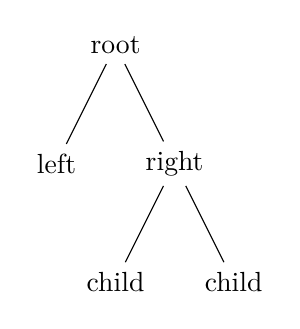
\begin{tikzpicture}
\node {root} 
child {node {left}} 
child {node {right} 
child {node {child}} 
child {node {child}}};
%!\caption{this is a figure}
%!\label{figure1}
\end{tikzpicture}
%  \caption{A picture}
\end{figure}
\end{document}

\hypertarget{tree-essai}{%
\subsection{tree essai}\label{tree-essai}}

\[latex
\begin{figure}
\node {root}
child {node {left}}
child {node {right}
child {node {child}}
child {node {child}}};
%!\caption{this is a figure}
%!\label{figure1}
  \caption{A picture}
  \end{figure}\]

\begin{Shaded}
\begin{Highlighting}[]
\CommentTok{\# \#td\textless{}{-}tempdir()}
\CommentTok{\# td\textless{}{-}getwd()}
\CommentTok{\# tf\textless{}{-}file.path(td,\textquotesingle{}example.tex\textquotesingle{})}
\CommentTok{\# oldwd\textless{}{-}getwd()}
\CommentTok{\# setwd(td)}
\CommentTok{\# }
\CommentTok{\# tikz(tf,standAlone=T)}
\CommentTok{\# plot(1)}
\CommentTok{\# dev.off()}
\CommentTok{\# }
\CommentTok{\# tools::texi2dvi(tf,pdf=T)}
\CommentTok{\# system(paste(getOption(\textquotesingle{}pdfviewer\textquotesingle{}),file.path(td,\textquotesingle{}example1.pdf\textquotesingle{})))}
\CommentTok{\# setwd(oldwd)}
\end{Highlighting}
\end{Shaded}

\[latex
\begin{tabular}{ll}
A & B \\
A & B \\
\end{tabular}\]

\begin{Shaded}
\begin{Highlighting}[]
\NormalTok{model }\OtherTok{\textless{}{-}} \FunctionTok{lm}\NormalTok{(mpg}\SpecialCharTok{\textasciitilde{}}\NormalTok{.,mtcars)}
\NormalTok{ coef1 }\OtherTok{\textless{}{-}} \FunctionTok{coef}\NormalTok{(model)[[}\DecValTok{1}\NormalTok{]]}
\NormalTok{ coef2 }\OtherTok{\textless{}{-}} \FunctionTok{coef}\NormalTok{(model)[[}\DecValTok{2}\NormalTok{]]}
\end{Highlighting}
\end{Shaded}

\[latex \hat{Y}= 12.3033742 + -0.1114405 \cdot Length\]

%-Theoreme-%

\theoremstyle{definition}
\newtheorem{D}{Definition}
\newtheorem{B}{Beispiel}
\newtheorem{Satz}{Satz}
\newtheorem{N}{Notation}

%!Theoremstil definition mit Zeilenumbruch
\newtheoremstyle{break}
{\topsep}%
{\topsep}%
{\normalfont}%
{}%
{\bfseries}%
{.}%
{\newline}
{}%

\theoremstyle{break}
\newtheorem{R}{Regularität}
\newtheorem{Bsp.}[B]{Beispiel}
\newtheorem{Sch}{Schema}

%!forest-Baumdiagramm: Pittner-Notation
\newcommand{\lingforestpittner}[3]{%
    \noindent\makebox[\textwidth]{
        \begin{forest}
            where n children=0{tier=word}{},
            for tree={l=#1pt}
            []
    \end{forest}}
}

%-Klammer-Notation (Pittner)-%

%!Klammern
\newcommand{\klammer}[2]{[#1]\textsubscript{\textbf{#2}}}
\newcommand{\Klammer}[2]{$\biggl[$#1$\biggr]$\textsubscript{\textbf{#2}}}
\newcommand{\KKlammer}[2]{$\Biggl[$#1$\biggr]$\textsubscript{\textbf{#2}}}
\newcommand{\pos}[1]{\textsubscript{\textbf{#1}}}

%!Grüne Klammern
\newcommand{\greenklammer}[2]{\textcolor{dartmouthgreen}{[}#1\textcolor{dartmouthgreen}{]}\textsubscript{\textbf{#2}}}
\newcommand{\greenKlammer}[2]{$\color{dartmouthgreen}\biggl[$#1$\color{dartmouthgreen}\biggr]$\textsubscript{\textbf{#2}}}
\newcommand{\greenKKlammer}[2]{$\color{dartmouthgreen}\Biggl[$#1$\color{dartmouthgreen}\Biggr]$\textsubscript{\textbf{#2}}}
%\newcommand{\greenpos}[1]{\textsubscript{\textbf{\textcolor{dartmouthgreen}{#1}}}}
\newcommand{\green}[1]{\textcolor{dartmouthgreen}{#1}}

%!Klammern: Übungen
\newcommand{\exklammer}[1]{[#1]\textsubscript{\subleer}}
\newcommand{\exKlammer}[1]{$\biggl[$#1$\biggr]$\textsubscript{\subleer}}
\newcommand{\exKKlammer}[1]{$\Biggl[$#1$\biggr]$\textsubscript{\subleer}}

%!Leerstelle im Subskript
\newcommand{\subleer}{\textsubscript{\textlarger[4]{\_}}}

%-Skripte-%

%!Oberskript
\newcommand{\oberskript}[2]{[$\overset{\textbf{#2}}{\text{#1}}$]}

%!Unterskript
\newcommand{\unterskript}[2]{$\underset{\textbf{#2}}{\text{\ul{#1}}}$}


%-Baumdiagramm-Notation-%

%!forest-Baumdiagramm: Standard
%!forest-Baumdiagramm: Standard
\newcommand{\lingforest}[2]{%
    \noindent\makebox[\textwidth]{
        \begin{forest}
            where n children=0{tier=word}{},
            for tree={l=#1pt}
            #2
    \end{forest}
    }
}

\begin{figure}[h]\label{figure01} 
\lingforest{30}{%
[PP, dashed
    [AdvP|NP|, dashed
        [links, no edge, tier=3]
    ]
    [\textbf{P},dashed,tier=1
        [auf, no edge, tier=2
            [neben, no edge, tier=3,
                [ins, no edge, tier=4]
            ]
        ]
    ]
    [NP, dashed,tier=1
        [der Einfahrt, no edge, tier=2
            [der Einfahrt, no edge, tier=3
                [Gebäude, no edge, tier=4]
            ]
        ]
    ]
]
}
%\end{figure}
%\end{forest}
\caption{fenced forest}
\end{figure}

%try if command declaration of above block can be used within this block


\vbox{%
\begin{Sch}[Präpositionalphrase (PP)]
\lingforest{30}{%
[PP, circle, draw
    [AdvP|NP|\\$\ldots$, circle, draw, dashed
        [links, no edge, tier=3]
    ]
    [\textbf{P}, circle, draw, tier=1
        [auf, no edge, tier=2
            [neben, no edge, tier=3,
                [ins, no edge, tier=4]
            ]
        ]
    ]
    [NP, circle, draw, tier=1
        [der Einfahrt, no edge, tier=2
            [der Einfahrt, no edge, tier=3
                [Gebäude, no edge, tier=4]
            ]
        ]
    ]
]
}
%\caption{with declared captions}

\end{Sch}
}

\begin{figure}[h]\label{figure01} 
\centering
\begin{forest}
[PP, dashed, tier=1
    [AdvP|NP, dashed,tier=2[
    links, dashed, tier=3]]
    [PP, dashed, tier=2
    [neben, dashed, tier=3]]
    [NP, dashed,tier=2
    [der Einfahrt, dashed, tier=3]]
]
%\end{figure}
\end{forest}
\caption{fenced forest}
\end{figure}

\hypertarget{waldbuxe4ume-usw.}{%
\subsubsection{wald/bäume usw.}\label{waldbuxe4ume-usw.}}

\hypertarget{another-baum}{%
\subsection{another baum}\label{another-baum}}

\[latex  
\begin{tikzpicture}
\node {root} 
child {node {left}} 
child {node {right} 
child {node {child}} 
child {node {child}}};
%!\caption{this is a figure}
%!\label{figure1}
\end {tikzpicture}\]

\hypertarget{baum-fenced-1}{%
\subsection{baum fenced}\label{baum-fenced-1}}

\begin{figure}[h]\label{figure1}
\centering

\begin{tikzpicture}
\node {root} 
child {node {left}} 
child {node {right} 
child {node {child}} 
child {node {child}}};
%!\caption{this is a figure}
%!\label{figure1}
  \end{tikzpicture}
  \caption{A picture}
  \end{figure}

\[latex  
We are working on
\begin{tikzpicture}
\draw (-1.5,0) -- (1.5,0);
\draw (0,-1.5) -- (0,1.5);
\end{tikzpicture}\]

\hypertarget{r-markdown}{%
\subsection{R Markdown}\label{r-markdown}}

This is an R Markdown document. Markdown is a simple formatting syntax
for authoring HTML, PDF, and MS Word documents. For more details on
using R Markdown see \url{http://rmarkdown.rstudio.com}.

When you click the \textbf{Knit} button a document will be generated
that includes both content as well as the output of any embedded R code
chunks within the document. You can embed an R code chunk like this:

\begin{Shaded}
\begin{Highlighting}[]
\FunctionTok{summary}\NormalTok{(cars)}
\end{Highlighting}
\end{Shaded}

\begin{verbatim}
##      speed           dist       
##  Min.   : 4.0   Min.   :  2.00  
##  1st Qu.:12.0   1st Qu.: 26.00  
##  Median :15.0   Median : 36.00  
##  Mean   :15.4   Mean   : 42.98  
##  3rd Qu.:19.0   3rd Qu.: 56.00  
##  Max.   :25.0   Max.   :120.00
\end{verbatim}

\hypertarget{including-plots}{%
\subsection{Including Plots}\label{including-plots}}

You can also embed plots, for example:

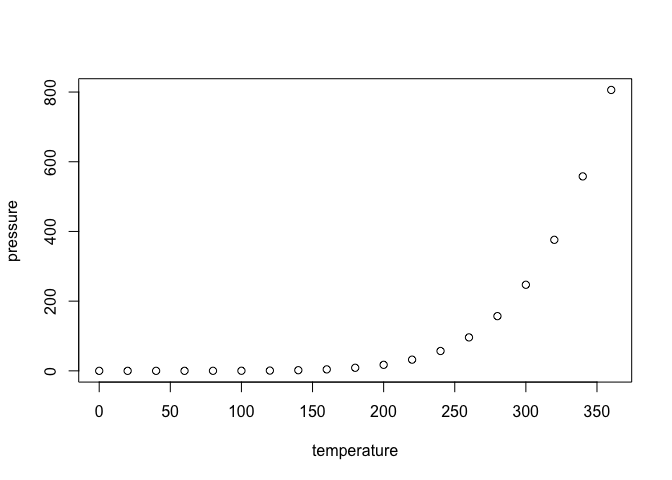
\includegraphics{tree_essai_files/figure-latex/pressure-1.pdf}

Note that the \texttt{echo\ =\ FALSE} parameter was added to the code
chunk to prevent printing of the R code that generated the plot.

\end{document}
